\documentclass{article}
\usepackage[utf8]{inputenc}
\usepackage{graphicx}
\usepackage[a4paper, total={8in, 10.5in}]{geometry}
\usepackage{rotating}
\usepackage{afterpage}
\usepackage{url}

\usepackage{algorithm}
\usepackage{algpseudocode}

\usepackage{amsmath}




\title{Numerical Analysis of Convection in the Inner Core (DRAFT)}
\author{Maximilian Williams}
\date{September 2021}

\begin{document}

\maketitle

\begin{abstract}
	Convection in the Earth's inner core has been a contentious topic in geoscience. Recently, it has been proposed through siesmic observations that Earths inner core is convecting. Here we numerically model convection in the Inner core, using the streamfunction-vorticity formulation and lattice boltzman method in 2-dimensions. 
	
 
\end{abstract}

\section*{Introduction}
In this report, we use two vastly different numerical tehcniques, the vorticity-streamfunction method and the Thermal Lattice Boltzman Method to simulate convection in an internally heated, self-gravitating bousiniesque fluid. Two codes are produced in python using the streamfunction-vorticity formulation in cartesian and polar coordinates. A single Thermal Lattice Boltzman Method (TLBM) code is produced in goLang. The python codes use limited libraries such as numpy while the goLang code uses only inbuilt libraries math, random numbers etc... 

Plan:
I want to also talk about why this is actually important, why is this something that is worth studying
\newline
Here I want to introduce the physics of what I want to talk about. I want to introduce 
the basic equations that I will use.
\newline






\subsubsection*{Governing Equations}
{\it{In this section I introduce the physics of the problem; the governing equations that we wish to numerically solve.}}
\vspace{0.3cm}
\newline
\noindent Throughout analysis we describe the fluid in the Eularian frame under a graviational acceleration $\vec{g}$ which may vary in space. We give each location in the fluid a velocity $\vec{u}$ and density $\rho$ that vary in space $\vec{x}$ and time $t$. We assume the fluids viscosity $\mu$, thermal diffusivity $\kappa$ and specific heat capacity $C_p$ are all constants. By conserving fluid momentum, we produce the navier stokes equation:
\begin{equation}
	\rho \frac{D \vec{u}}{D t} = \rho \vec{g} - \nabla p + \mu \nabla^2 \vec{u},
	\label{NSE}
\end{equation}
where $\frac{D}{D t} = \frac{\partial }{\partial t} + (\vec{u} \cdot \nabla)$ is the material derivative, $p$ the pressure of the fluid and $\nabla$ the del operator. The dynamics of fluid temperature $T$ are described the inhomoenous advection diffusion equation:
\begin{equation}
	\frac{D T}{D t} = \kappa \nabla^2 T + \frac{Q}{C_v \rho},
	\label{adeT}
\end{equation}
where $Q$ is the heat generated per unit volume per unit time, $C_v$ the specific heat at constant volume and $\rho$ the fluid density. The density of the fluid $\rho$ is assumed to vary linearly in temeprature according to the equation of state:
\begin{equation}
	\rho = \rho_0 (1- \alpha(T - T_0)),
	\label{equation of state}
\end{equation}
where $\alpha$ is the volumetric expansion coeffecient and $\rho_0$ the density at a reference temperature $T_0$.
Through siesmic imaging, variations in inner core density are $<< 1 \%$. We also assume that the inner cores evolution occures over geologic timescales, and as such take $\vec{u}$ to be first order. These assumptions allow us to make the slow flow boussinesq approximation to equation \ref{NSE}:
\begin{equation}
	\frac{\partial \vec{u}}{\partial t} = \frac{\rho'}{\rho} \vec{g} -   \frac{\nabla p'}{\rho_0} + \nu \nabla^2 \vec{u},
	\label{NSE slow + boussinesq}
\end{equation}
where $\rho'=-\alpha(T - T_0)$, $\nu$ the kinomatic viscosity $\nu = \frac{\mu}{\rho_0}$ and $p'$ a first order pertibation to the background pressure $p_0$.
\newline
The Earths




\subsection*{Numerical Methods}

{\it{Two numerical methods are introduced for solving the thermal convection problem, the Lattice Boltzman Method and the streamfunction-vorticity formulation. }}

\subsubsection*{Streamfunction-Vorticity formulation}
{\it{Here I introduce the streamfunction-vorticity method for use in 2 dimensions and use it to eliminate pressure terms in \ref{NSE slow + boussinesq} and \ref{adeT} in cartesian and polar geometries giving a set of numerically solvable equations.}}
\vspace{0.3cm}
\newline
\noindent The streamfunction-vorticity formulation is a popular method for analytical and simple numerical analysis of incompressable fluids in two dimensions. Its main advantage is its elimination of all pressure terms, which would typically require iterative techniques to solve, as is used in the SIMPLE algorithm. However, the streamfunction-vorticity method is limited to 2-dimensional or 3-dimensional symmetric flows and so has limited applicability.

We define two scalar quantities, the vorticity $\omega$ and the streamfunction $\psi$. The vorticity $\omega$ is given by:
\begin{equation}
	\omega = (\nabla \times \vec{u})_z,
	\label{omega}
\end{equation}
where the $z$ subscript denotes the component out of the plane. We also define a streamfunction $\psi$ by:
\begin{equation}
	\omega = - \nabla^2 \psi.
	\label{psi}
\end{equation}
Given a coordinate system, and a clever definition of $\vec{u}$ we can rewrite equations \ref{adeT} and \ref{NSE slow + boussinesq} in terms of $\omega$ and $\psi$ rather than $\vec{u}$ and $p$. In cartesian coordinates $(x,y)$ we pick 
\begin{equation}
	u = \frac{\partial \psi}{\partial y}, v = -\frac{\partial \psi}{\partial x},
	\label{cartesian velocities}
\end{equation}
allowing us to write equations \ref{adeT} and \ref{NSE slow + boussinesq} as:
\begin{equation}
	\frac{\partial T}{\partial t} + \frac{\partial \psi}{\partial y} \frac{\partial T}{\partial x} - \frac{\partial \psi}{\partial x} \frac{\partial T}{\partial y} = \kappa \nabla^2 T + \frac{Q}{\rho_0 C_v}
	\label{adeT sfvt cartesian}
\end{equation}
\begin{equation}
	\frac{\partial w}{\partial t} = -\frac{g_y}{\rho_0} \frac{\partial \rho'}{\partial x} + \nu \nabla^2 \omega
	\label{NSE slow + boussinesq sfvt cartesian}
\end{equation}
Similary, in polar coordinates (r, $\theta$) we pick:
\begin{equation}
	u = \frac{1}{r} \frac{\partial \psi}{\partial \theta}, v = -\frac{\partial \psi}{\partial r},
	\label{polar velocities}
\end{equation}
giving:
\begin{equation}
	\frac{\partial T}{\partial t} + \frac{1}{r} \frac{\partial \psi}{\partial \theta} \frac{\partial T}{\partial r} - \frac{1}{r} \frac{\partial \psi}{\partial r} \frac{\partial T}{\partial \theta} = \kappa \nabla^2 T + \frac{Q}{\rho_0 C_v}
	\label{adeT sfvt polar}
\end{equation}
and,
\begin{equation}
	\frac{\partial \omega}{\partial t} = - \frac{g_r}{\rho_0 r} \frac{\partial \rho'}{\partial \theta} +\nu \nabla^2 \omega.
	\label{NSE slow + boussinesq sfvt polar}
\end{equation}
A full derivation of equations \ref{adeT sfvt cartesian}, \ref{NSE slow + boussinesq sfvt cartesian}, \ref{adeT sfvt polar}, \ref{NSE slow + boussinesq sfvt polar} are given in appendix.
Importantly, our definitions of $u$ and $v$ in equations \ref{cartesian velocities} and \ref{polar velocities} satisify equation \ref{omega} and \ref{psi}. Equations \ref{psi}, \ref{adeT sfvt cartesian}, \ref{NSE slow + boussinesq sfvt cartesian} for the cartesian case and \ref{psi}, \ref{adeT sfvt polar}, \ref{NSE slow + boussinesq sfvt polar} for the polar case can be directly solved.

\subsubsection*{Solving the streamfunction-vorticity equations}
{\it{The finite difference method used for solving the streamfunction-vorticity-formulated governing equations is shown}}
\vspace{0.3cm}
\newline
\noindent We first discritize our domain $\mathcal{D}$. In the cartesian case, we use $(x_i,y_j)=(i \Delta x, j \Delta y)
$ with integers $i$ and $j$ satisfying $0\leq i < N_x$ $0 \leq j < N_y$. In the polar case, we use $(r_i, \theta_j)= (R_0 
+ i \Delta r, j 
\Delta \theta)$ again with  $0 \leq i < N_r$ and $0 \leq j < N_{\theta}$. We impose $\Delta \theta = \frac{2 \pi}
{N_{\theta} - 1}$ for consistancy with $\theta$-periodic boundary conditions and an inner radius $R_0$ in polar 
coordinates to avoid 
singularities generated by $r=0$. We also discritize time $t$ by $t_n = n \Delta t$. For a function $f$, we use 
$f^n_{i,j}$ to mean $f$ evaluated at time $n$ at position $(x_i,y_j)$ in cartesian coorindates or $(r_i, \theta_j)$ in 
polar coordinates. 
\newline
To approximate derivatives we use a finite difference approach. All time derivatives are approximated by forward difference:
\begin{equation}
	\frac{\partial f}{\partial t} = \frac{f^{n+1} - f^{n}}{\Delta t}
	\label{forward time difference}
\end{equation}
Second order space derivatives are apprimxated by a central difference:
\begin{equation}
	\frac{\partial^2 f_{i,j}}{\partial {x_1}^2} = \frac{f_{i+1,j} - 2 f_{i,j} + f_{i-1,j}}{{\Delta x_1}^2},
\end{equation}
\begin{equation}
	\frac{\partial^2 f_{i,j}}{\partial {x_2}^2} = \frac{f_{i,j+1} - 2 f_{i,j} + f_{i,j-1}}{{\Delta x_2}^2},
\end{equation}
where $x_1$ is the first coordinate and $x_2$ is the second coordinate. For example, in cartesian coordinates $(x,y)$, we would have $x_1=x$ and $x_2=y$. 
For non advection terms, we approximate first order spatial derivaitves by:
\begin{equation}
	\frac{\partial f_{i,j}}{\partial x_1} = \frac{f_{i+1,j} - f_{i-1,j}}{2{\Delta x_1}},
\end{equation}
and
\begin{equation}
	\frac{\partial f_{i,j}}{\partial x_2} = \frac{f_{i,j+1} - f_{i,j+1}}{2{\Delta x_2}}.
\end{equation}
For advection terms, of the form $a \frac{\partial f_{i,j}}{\partial x_1}$ we employ a first order godanov scheme:
\begin{equation}
	a \frac{\partial f_{i,j}}{\partial x_1} = \frac{1}{\Delta x} ( \mid a\mid (  \frac{1}{2} f_{i+1,j} - \frac{1}{2} f_{i-1,j}   ) - a ( \frac{1}{2} f_{i+1,j} -f_{i,j} - \frac{1}{2} f_{i-1,j} )).
\end{equation}
This scheme is always downstream, regardless of the direction of the advecting field $a$.
\newline
Other more accurate, but substantually more complex methods for solving these equations, particularlly the advection equation exists such as the semi-lagrange crank-nicolson scheme.
\newline
To solve the streamfuntion-vorticity equations we assume a starting vorticity $\omega$ on our domain $\mathcal{D}$. We then apply the Jacobi method to solve equation \ref{psi} for $\psi$ on the interior of the domain which we call $\mathcal{D}'$. 
Using $\psi$ we update $T$ on $\mathcal{D}'$ using equation \ref{adeT sfvt cartesian} (or \ref{adeT sfvt polar} for polar). Finally, $\omega$ is updated on $\mathcal{D}'$ using 
equation \ref{NSE slow + boussinesq sfvt cartesian} (\ref{NSE slow + boussinesq sfvt polar} for polar). This process is repeated.

\subsubsection*{The Jacobi Method}
{\it{Here a basic numerical method for solving the Poisson equation, the Jacobi method is outlined.}}
We cannot solve for $\psi$ explicitly in equation \ref{psi}. Instead we use an iterative jacobi method. In cartesian coordinates, equation \ref{psi} is:
\begin{equation}
	\omega_{i,j} = \frac{\psi_{i+1,j} - 2 \psi_{i,j} + \psi_{i-1,j}  }{{\Delta x}^2} + \frac{\psi_{i,j+1} - 2 \psi_{i,j} + \psi_{i,j-1}  }{{\Delta y}^2}
	\label{psi disc}
\end{equation}
Rearanging for $\psi$
\begin{equation}
	\psi_{i,j} = \frac{{\Delta x}^2 {\Delta y}^2  }{2({\Delta x}^2  + {\Delta y}^2)} (\frac{\psi_{i+1,j} +\psi_{i-1,j} }{{\Delta x}^2} + \frac{\psi_{i,j+1} +\psi_{i,j-1}  }{{\Delta y}^2 }  + \omega_{i,j}).
	\label{psi from omega}
\end{equation}
We then use the result of $\psi_{i,j}$ back into equation \ref{psi from omega} to solve for $\psi_{i,j}$ iterately as shown in equation \ref{psi iterative}:
\begin{equation}
	\psi_{i,j}^{(k+1)} = \frac{{\Delta x}^2 {\Delta y}^2  }{2({\Delta x}^2  + {\Delta y}^2)} (\frac{\psi_{i+1,j}^{(k)} +\psi_{i-1,j}^{(k)}  }{{\Delta x}^2} + \frac{\psi_{i,j+1}^{(k)} +\psi_{i,j-1}^{(k)}  }{{\Delta y}^2 } + \omega_{i,j}).
	\label{psi iterative}
\end{equation}
Where the superscript $(k)$ means the result of the $k^{th}$ iteration of the above equation and this operation us applied to all points in $\mathcal{D}'$.
 We terminate this iterative method once the error $\sum_{(i,j) \in \mathcal{D'}} \mid \psi_{i,j}^{(k+1)} - \psi_{i,j}^{(k)} \mid$ gets suffeciently small. A similar method is applied to the polar coordinate case. 
 



\subsubsection*{Solution Stability and Accuracy}
%% Here I want to look at the stabiliy of this method

 


\subsubsection*{Lattice Boltzman Method}
{\it{In this section I give a brief introduction to the Lattice Boltzman Method and why its different from most numerical tehcniques. I introduce a 2-dimensional lattice D2Q9 and discribe the Thermal Lattice Boltzman method (TLBM) which is employed by my numerical solution to simulate convection.}}
\vspace{0.3cm}

\noindent The Lattice Boltzman Method (LBM) is a generalization of a Lattice Gas Automata (LGA), which are themselves a 
specialized Automata for simulating fluid flows. These Automata methods like common fluid simulation techniques 
discritize space and time. They directly simulate the state of particles or their distributions and evolve in time 
accoring to rules which give the desired macroscopic fluid properties as an emergent effect. This is fundamentally 
different from typical approaches which amount to directly numerically solving a set of partial differential equations.
\newline
\noindent To discritize space, we place nodes at locations $(x_i,y_j)=(i,j)$ with $i,j$ integers. Each node has attached to it a latitce, here the D2Q9 lattice shown in figure \ref{D2Q9}. The lattice defines unit vectors $\vec{e}_i$, $i \in \{ 0,1,2,3,4,5,6,7,8 \}$. In addition, each direction $e_i$ gets a weight $w_i$. In the D2Q9 lattice these are:
\begin{equation*}
w_i = \begin{cases}
          \frac{4}{9} \quad &\text{if}  \ i=0 \\
          \frac{1}{9} \quad &\text{if} \ i=1,2,3,4 \\
          \frac{1}{36} \quad &\text{if} \ i=5,6,7,8 \\
     \end{cases}.
\end{equation*}
\begin{figure}[h!]
	\centering
	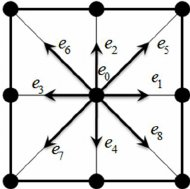
\includegraphics{D2Q9Lattice.jpg}
	\caption{D2Q9 Lattice. Black notes repressent lattice points, vectors $e_0,..,e_8$ are the lattice vectors. Image sourced from \cite{khazaeli2015ghost}}
	\label{D2Q9}
\end{figure}
\noindent We wish to simulate convection. For this, we require the particle motion and the internal energy throughout the lattice. We define two distribution functions $f_{\alpha}(\vec{x}, t)$ and $g_{\alpha}(\vec{x}, t)$ denoting the particle and internal energy distributions along direction $\alpha$ at lattice points $\vec{x}$ and times $t$. The direction can be thought of as the direction of flow for particles or energy. Each timestep there are two steps to updating $f$ and $g$, a common streaming step:
\begin{equation}
	f_{\alpha}(\vec{x} + \vec{e}_\alpha, t + \Delta t) = f_{\alpha}(\vec{x}, t),
	\label{streaming step}
\end{equation}
and different collision steps:
\begin{equation}
	f_{\alpha}(\vec{x} + \vec{e}_{\alpha}, t + \Delta t) = f_{\alpha}(\vec{x}, t) + \frac{1}{\tau_f} (f^{eq}_{\alpha}(\vec{x}, t)  - f_{\alpha}(\vec{x}, t)) + F_{\alpha}
	\label{f collision step}
\end{equation}
\begin{equation}
	g_{\alpha}(\vec{x} + \vec{e}_{\alpha}, t + \Delta t) = g_{\alpha}(\vec{x}, t) + \frac{1}{\tau_g} (g^{eq}_{\alpha}(\vec{x}, t)  - g_{\alpha}(\vec{x}, t)) + G_{\alpha}.
	\label{g collision step}
\end{equation}
Here $F_{\alpha}$ and $G_{\alpha}$ are the forcing terms terms and $f^{eq}_{\alpha}$ and $g^{eq}_{\alpha}$ are equilibrium distributions. The relaxation times $\tau_f$ and $\tau_g$ are related to the macroscopic thermal diffusivity ($\kappa$) and kinematic viscousity $\nu$ by:
\begin{equation}
	\tau_g = \frac{3 \kappa}{S^2 \Delta t} + \frac{1}{2}
\end{equation}
and,
\begin{equation}
	\tau_f = \frac{3 \nu}{S^2 \Delta t} + \frac{1}{2}.
\end{equation}
The equilibrium distributions are given by the BKG approximation:
\begin{equation}
	f^{eq}_{\alpha}(\vec{x}, t)  = \rho w_{\alpha} (1 + 3 \frac{\vec{e}_{\alpha} \cdot \vec{u}}{s^2} + \frac{9}{2} \frac{(\vec{e}_{\alpha} \cdot \vec{u}  )^2}{c^4} - \frac{3}{2} \frac{\vec{u} \cdot \vec{u}}{c^2}  ),
\end{equation}
\begin{equation}
	g^{eq}_{\alpha}(\vec{x}, t)  = \epsilon \rho w_{\alpha} (1 + 3 \frac{\vec{e}_{\alpha} \cdot \vec{u}}{s^2} + \frac{9}{2} \frac{(\vec{e}_{\alpha} \cdot \vec{u}  )^2}{c^4} - \frac{3}{2} \frac{\vec{u} \cdot \vec{u}}{c^2}  ),
\end{equation}

Here $\rho$, $\epsilon$ and $\vec{u}$ are the macroscopic density, internal energy and velocity given by:
\begin{equation}
	\rho = \sum_{i=0}^{8} f_{i},
	\label{LBM rho}
\end{equation}
\begin{equation}
	\rho \vec{u} = \sum_{i=0}^{i=8} f_{i} \vec{e}_{i}
	\label{LBM u}
\end{equation}
and,
\begin{equation}
	\rho \epsilon = \sum_{i=0}^{i=8} g_{i}.
	\label{LBM ep}
\end{equation}
The forcing terms $F_i$ and $G_i$ are problem dependent. For thermal convection $G_i=0$ and $F_i$ is a gravitational term ${\Delta f}_{\alpha}$:
\begin{equation}
	{\Delta f}_{\alpha} = - w_{\alpha} \rho \alpha \epsilon \frac{\vec{e}_{\alpha}}{\mid \vec{e}_{\alpha} \mid} \cdot \vec{g} \frac{1}{\tau_{grav}},
\end{equation}
where $\mid \mid$ is the vector norm and $\vec{g}$ is the gravitational acceleration. Here $\tau_{grav}$ is the relaxation time for the gravitational field. We take $\tau_g=0.6$ here, following \cite{mora2017simulation}. The algorithm used to evolve the above TLBM equations is given in algorithm \ref{alg:TLBM}

\begin{algorithm}[h!]
\caption{Thermal Lattice Boltzman Algorithm}\label{alg:TLBM}
\begin{algorithmic}

\State $f_{\alpha} = \rho_0 w_{\alpha}$
\State $\epsilon = 0$
\State $\epsilon_b$
\State $\rho = 0$
\State $\vec{u} = 0$
\While{Simulation Running}
	\State $g_{\alpha} += \rho \epsilon_b w_{\alpha} $
	\If{$x-\vec{e}_{\alpha}$ is solid}
		\State $f_{\alpha}(x) = f_{\alpha'}(x)$
		\State $g_{\alpha}(x) = g_{\alpha'}(x)$
	\Else
		\State $f_{\alpha}(x) = f_{\alpha}(x - \vec{e}_{\alpha})$
		\State $g_{\alpha}(x) = g_{\alpha}(x - \vec{e}_{\alpha})$
	\EndIf
	\State $\rho = \sum_{i=0}^{i=8} f_{i}$
	\State $\vec{u} =\frac{(\sum_{i=0}^{i=8} f_{i} \vec{e}_{i})}{\rho} $
	\State $\epsilon = \frac{\sum_{i=0}^{i=8} g_{i}}{\rho}$
	\State $f^{eq}_{\alpha} = \rho w_{\alpha} (1 + 3 \frac{\vec{e}_{\alpha} \cdot \vec{u}}{s^2} + \frac{9}{2} \frac{(\vec{e}_{\alpha} \cdot \vec{u}  )^2}{c^4} - \frac{3}{2} \frac{\vec{u} \cdot \vec{u}}{c^2})  $
	\State $g^{eq}_{\alpha}(\vec{x}, t)  = \epsilon \rho w_{\alpha} (1 + 3 \frac{\vec{e}_{\alpha} \cdot \vec{u}}{s^2} + \frac{9}{2} \frac{(\vec{e}_{\alpha} \cdot \vec{u}  )^2}{c^4} - \frac{3}{2} \frac{\vec{u} \cdot \vec{u}}{c^2}  ) $ 
	\State ${\Delta f}_{\alpha} = - w_{\alpha} \rho \alpha \epsilon \frac{\vec{e}_{\alpha}}{\mid \vec{e}_{\alpha} \mid} \cdot \vec{g}$
	\State $\tau_g = \frac{3 \kappa}{S^2 \Delta t} + \frac{1}{2}$
	\State $\tau_f = \frac{3 \nu}{S^2 \Delta t} + \frac{1}{2}$
	\State $f_{\alpha} = f_{\alpha} + \frac{f^{eq}_{\alpha}-f_{\alpha}}{\tau_f} + {\Delta f}_{\alpha}$
	\State $g_{\alpha} = g_{\alpha} + \frac{g^{eq}_{\alpha}-g_{\alpha}}{\tau_g}$
\EndWhile
\end{algorithmic}
\end{algorithm}

\subsubsection*{Boundary Conditions}
%% here I want to go over the boundary conditions that I used 
%% I might not have space to go over exactly how I did this here. Maybe that can be in the appendix.
In both streamfunction-vorticity codes, boundaries were assumed to be fluid-impermiable, non-slip and insulating. In the Lattice Boltzman code, ''bounce 
back" boundary condition was used. This is a fluid-impermiable, insulating and slip boundry.

\section*{Advection tests}
{\it{Here I pressent some simple tests that show how accurately my advection scheme is performing in both geometries.}}
\vspace{0.3cm}
\noindent Next we tested the accuarcy of the advection schemes. Thermal diffusivity ($\kappa$) and thermal expansion ($\alpha$) were set to zero to avoid convection. The fluid was set to temperature 0 (arb. units) except a small segment which was set to $1$ shown in yellow top left of figure \ref{polar periodic advection}, \ref{polar diagonal advection}, \ref{cartesian periodic advection}, \ref{cartesian diagonal advection}. A streamfunction $\psi_c$ was enforced to produce diagonal back and forth motion or a continous horizontal or azimuthal motion to cross a periodic boundary. Details of the streamfunctions used are given in appendix.

\begin{figure}[h!]
	\centering
	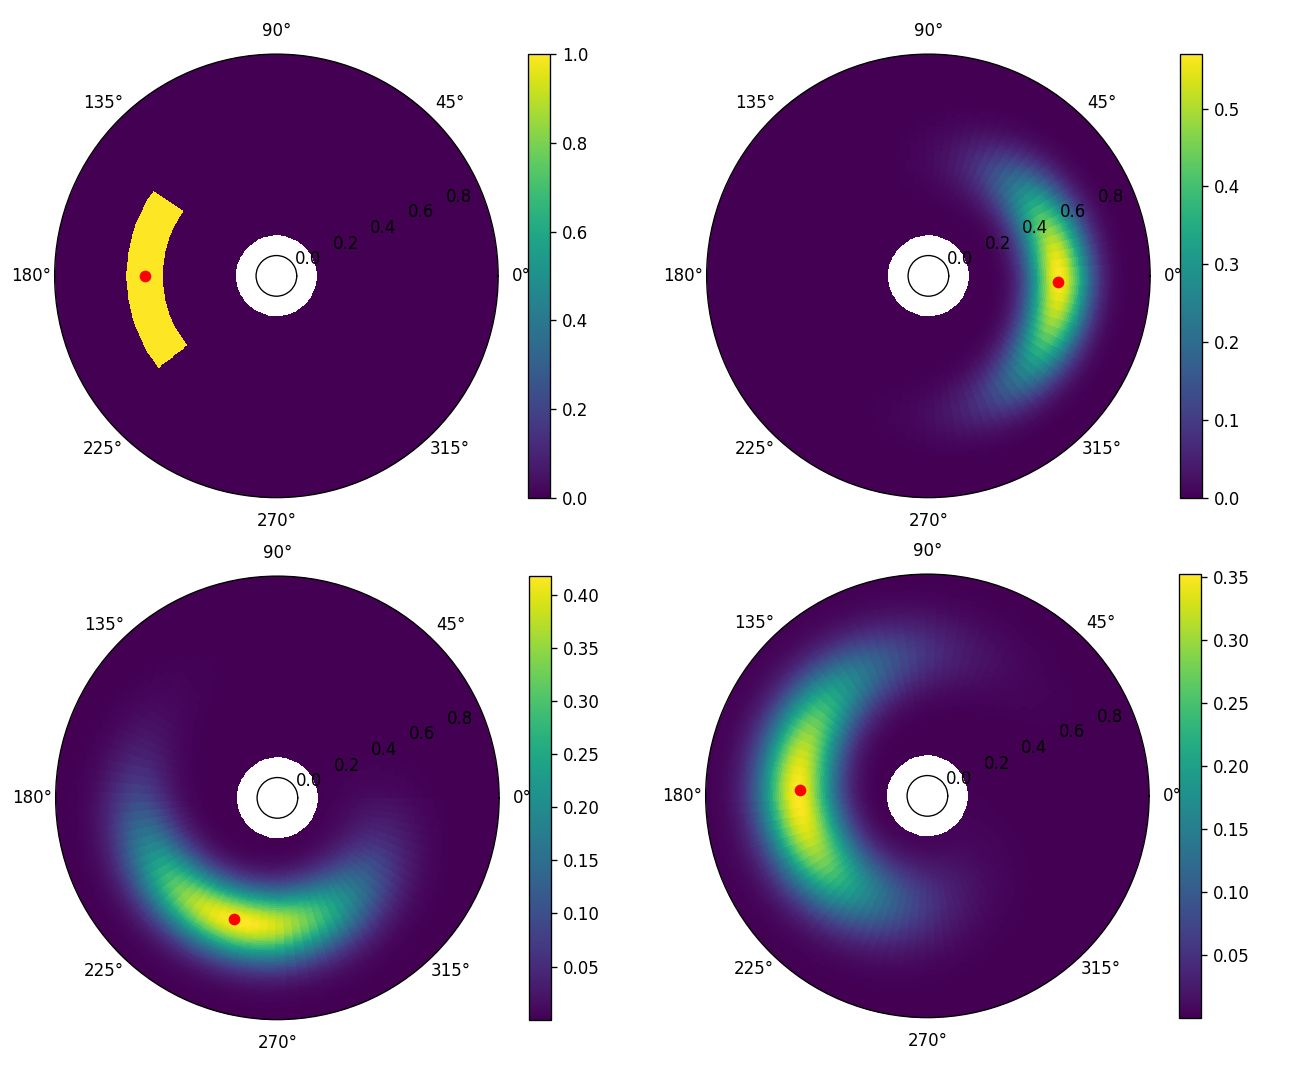
\includegraphics{polarPeriodic/PolarPeriodicFigure.jpg}
	\caption{Polar azimuthal advection test. Temperature (color) is plotted in polar space. Red dot indicates temperature weighted mean position within 
	the fluid and is taken as the location of the temperature 1 zone. Fluid is advected by an anticlockwise flow. Cronological order is Top left, top right, bottom left, bottom right. Top left shows the initial condition. Top right shows advection across periodic boundary. Bottom left is state when an exact scheme would have returned to the original position. Bottom right is the final state after being advected around one rotation.}
	\label{polar periodic advection}
\end{figure}
\begin{figure}[h!]
	\centering
	\includegraphics{polarDiagonal/PolarDiagonalFigure.jpg}
	\caption{ Polar coorindate diagonal advection test. Similar convection used to figure \ref{polar periodic advection}. Fluid is diagonally advected over a time $t$ from the initial state (top left) to top right. The advection field is reversed for time $2t$ giving bottom left. The field is reversed again producing bottom right.}
	\label{polar diagonal advection}
\end{figure}
 
\begin{figure}[h!]
	\centering
	\includegraphics{cartesianPeriodic/CartesianPeriodicFigure.jpg}
	\caption{Cartesian coordinate advection test accross a periodic boundary. Convention similar to figure \ref{polar periodic advection}.}
	\label{cartesian periodic advection}
\end{figure}

\begin{figure}[h!]
	\centering 
	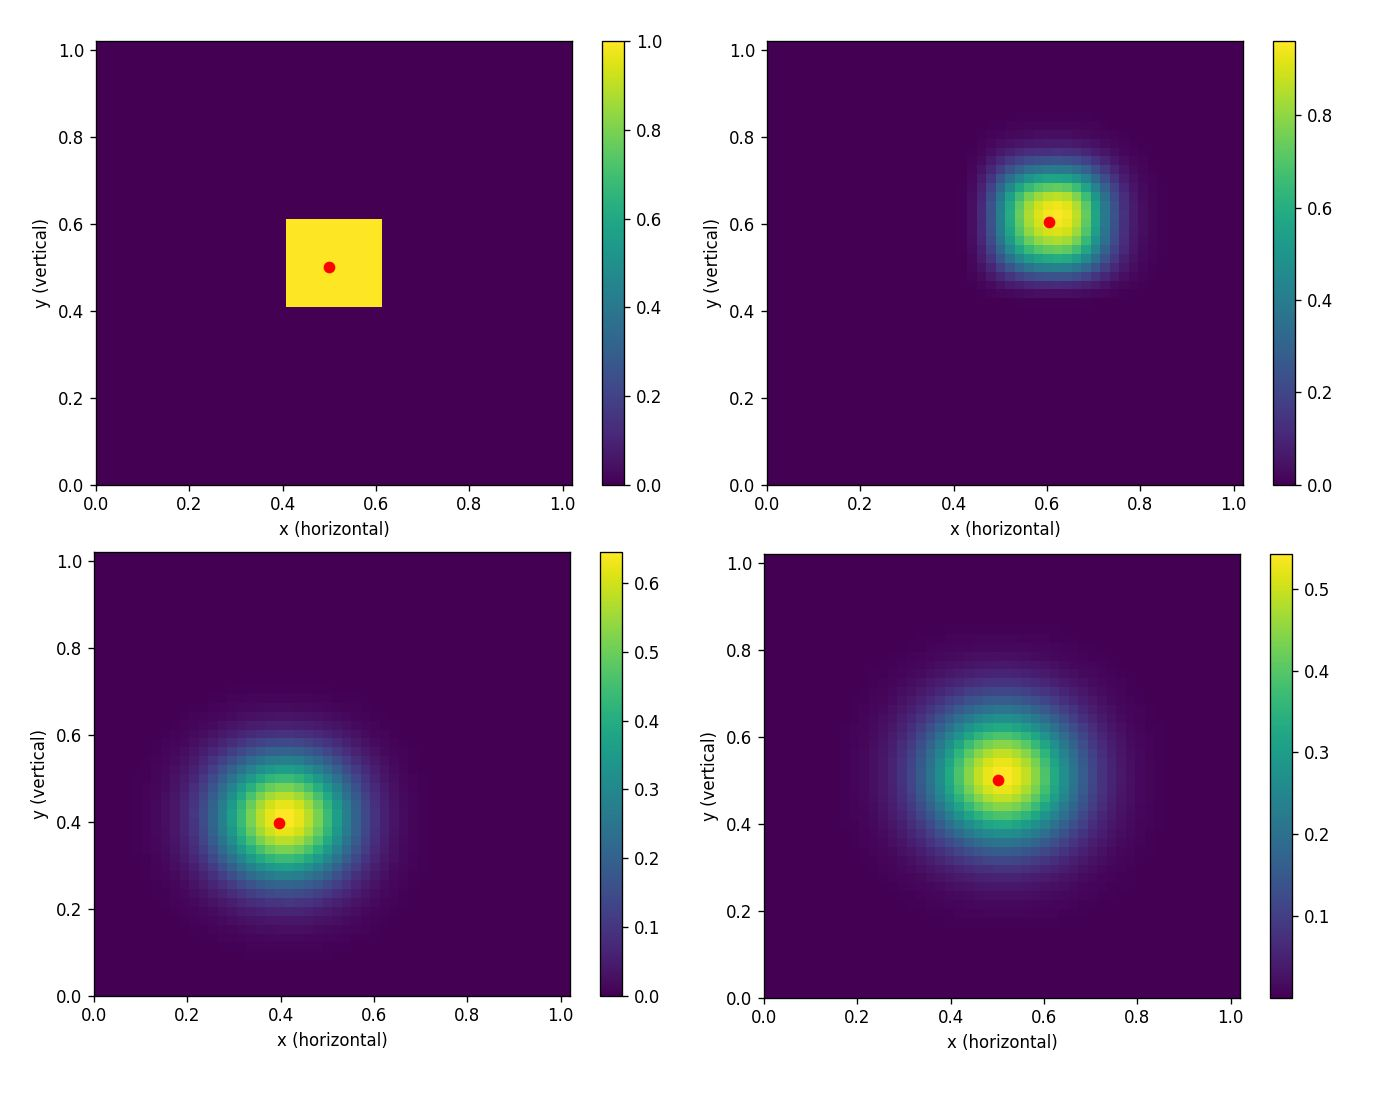
\includegraphics{cartesianDiagonal/CartesianDiagonalFigure.jpg}
	\caption{Cartesian diagonal advection test. Similar convention to figure \ref{polar diagonal advection}. }
	\label{cartesian diagonal advection}
\end{figure}

\noindent The advection results for both codes are similar. For the periodic advection test figures \ref{polar periodic advection} and \ref{cartesian periodic advection} the temperature 1 region was advected across the periodic boundary without additional distortion. The centroid (red dot) also lagged the advection field by $\approx 1 \%$ and $\approx 10 \%$ for the cartesian (figure \ref{cartesian periodic advection}) and polar case (figure \ref{polar periodic advection}) respectively. It is unknown why these differ substantually, but a probable cause is a smaller timestep used to produce the polar tests. In all cases, the bluring shows numerical diffusion which happens along the direction of the advection field as predicted by equation \ref{stability equation}. The discontinuity in temperature in figure \ref{polar diagonal advection} (bottom left) near the azimuthal 0 to 360 boundary is a result of setting a streamfunction with a disconinuity here. 


\section*{Simulations}

The cartesian and polar streamfunction-vorticity codes are limited in two 
distinct ways. The polar geometry of the 2-dimensional inner core is well 
suited to polar coorindates. However, by using polar coorindates, a 
singularity in the governing equations occures at the center 
$r \rightarrow 0$. For standard regularly spaced meshes as is used here, 
this causes the lattice spacing near the center to become infinicimal 
requiring small timesteps and large amounts of compute time. For this 
reason, the inner region of the polar domain is exlcuded leaving out a 
critical region in the simulation. In cartesian coorindates, there is no 
singularity and the full domain is included, however it becomes difficult 
to recreate the polar geometry and enforce boundary conditions. Because of 
this, we approximate the 2-dimensional inner core by ''unrolling" as shown 
in figure \ref{unrolling}, losing the affect of the polar geometry. 


\begin{figure}[h!]
	\centering
	
\includegraphics{frog.png}
	\caption{figure showing how the 2-dimensional polar domain is ''unrolled" into a 2-dimensional cartesian domain.}
	\label{unrolling}
\end{figure}

\subsection*{How much does the geometry matter}
{\it{In this section I compaire the results from the polar and cartesian streamfunction-vorticity codes with similar Prantl and Rayleigh number to see how the geometry affects convection.}}

A gravitational field linearly proportional to height and radius for the 
cartesian and polar codes respectively was set. A constant internal 
heating field $H$ was set for all but the upper $10 \%$ of both domains. A 
compensating heating field was set at the remaining top of the domain to 
balence the total heat generation. Note this heat field is different in 
the cartesian and polar cases. In all heating fields time-independent 
random flucations of $\approx 1 \%$ were set to faciliate instabilities.

\begin{figure}
	\centering
	
\includegraphics{frog.png}
	\caption{Internally Heated Convection comparison between cartesian 
	case (left) and polar case (right) $Pr=1, Ra=10^8$}
	\label{cartesian vs polar}
\end{figure}




\subsection*{How much does the central region matter?}








\subsection*{Thermal Lattice Boltzman Simulations}



\section*{Dicussion}


\section*{Conclusion}


\section*{Appendix}

\subsection*{Derivation of Graviational Field in a self gravitating fluid}
We assume that the Earth is homogenous accross polar and azimuthal variations. By applying Gauss's law to this that 


\subsection*{Some Scales that I used}
This is an important source here \cite{goluskin2016internally}.
\newline
We chose the following legnth scales for the problem. For length we used $d$, the height or radius of the domain, 
for timescale we used $\frac{d^2}{\kappa}$, for pressure we used $\frac{\rho_0 d^2}{\kappa}$, for temperature we used $\frac{d^2 H}{\kappa}$. 
I took the rayleigh number as $Ra = \frac{g \alpha H d^5}{\nu \kappa^2}$ and the Prantl number $Pr = \frac{\nu}{\kappa}$. I additionally define a timescale for transport via flow:
\begin{equation}
	\tau = \frac{\kappa \nu}{g \alpha H d^3}
\end{equation}




\bibliographystyle{abbrv}
\bibliography{ref.bib}





\end{document}
